\documentclass[12pt,a4paper]{report}
\usepackage[utf8]{inputenc}
\usepackage[spanish]{babel}
\usepackage{amsmath}
\usepackage{amsfonts}
\usepackage{amssymb}
\usepackage{graphicx}
\graphicspath{ {images/} }
\usepackage{color}

\definecolor{miverde}{rgb}{0,0.6,0}
\definecolor{migris}{rgb}{0.5,0.5,0.5}
\definecolor{mimalva}{rgb}{0.58,0,0.82}
\usepackage{listings}%Para insertar codigo de programacion
\lstset{ %
  backgroundcolor=\color{white},   % Indica el color de fondo; necesita que se añada \usepackage{color} o \usepackage{xcolor}
  basicstyle=\footnotesize,        % Fija el tamaño del tipo de letra utilizado para el código
  breakatwhitespace=false,         % Activarlo para que los saltos automáticos solo se apliquen en los espacios en blanco
  breaklines=true,                 % Activa el salto de línea automático
  captionpos=b,                    % Establece la posición de la leyenda del cuadro de código
  commentstyle=\color{miverde},    % Estilo de los comentarios
  deletekeywords={...},            % Si se quiere eliminar palabras clave del lenguaje
  escapeinside={\%*}{*)},          % Si quieres incorporar LaTeX dentro del propio código
  extendedchars=true,              % Permite utilizar caracteres extendidos no-ASCII; solo funciona para codificaciones de 8-bits; para UTF-8 no funciona. En xelatex necesita estar a true para que funcione.
  frame=single,	                   % Añade un marco al código
  keepspaces=true,                 % Mantiene los espacios en el texto. Es útil para mantener la indentación del código(puede necesitar columns=flexible).
  keywordstyle=\color{blue},       % estilo de las palabras clave
  language=c++,                 % El lenguaje del código
  otherkeywords={*,...},           % Si se quieren añadir otras palabras clave al lenguaje
  numbers=left,                    % Posición de los números de línea (none, left, right).
  numbersep=5pt,                   % Distancia de los números de línea al código
  numberstyle=\small\color{migris}, % Estilo para los números de línea
  rulecolor=\color{black},         % Si no se activa, el color del marco puede cambiar en los saltos de línea entre textos que sea de otro color, por ejemplo, los comentarios, que están en verde en este ejemplo
  showspaces=false,                % Si se activa, muestra los espacios con guiones bajos; sustituye a 'showstringspaces'
  showstringspaces=false,          % subraya solamente los espacios que estén en una cadena de esto
  showtabs=false,                  % muestra las tabulaciones que existan en cadenas de texto con guión bajo
  stepnumber=1,                    % Muestra solamente los números de línea que corresponden a cada salto. En este caso: 1,3,5,...
  stringstyle=\color{mimalva},     % Estilo de las cadenas de texto
  tabsize=2,	                   % Establece el salto de las tabulaciones a 2 espacios
  title=\lstname                   % muestra el nombre de los ficheros incluidos al utilizar \lstinputlisting; también se puede utilizar en el parámetro caption
}
\author{Elaborado por:\\\\Rivera Negrete Manuel Armando}
\date{28 de Junio del 2018}
\title{Universidad Nacional Autónoma de México\\Programa de Tecnología en Cómputo\\Lo que siempre quisiste saber de C\# y nunca te atreviste a preguntar}

\begin{document}
\maketitle
\tableofcontents
\cleardoublepage
\part*{¿Por qué aprender C\#?}

\part{C\# Básico}

\chapter{La arquitectura .NET}
\section{C\# y su lugar dentro de .NET}
C\# (leído <<C sharp>>) es un lenguaje de programación orientado a objetos desarrollado y estandarizado por Microsoft como partes de su plataforma .NET. Aunque esta plataforma permite desarrollar aplicaciones en otros lenguajes de programación, C\# ha sido creado específicamente para .NET, adecuando todas sus estructuras a las características y capacidades de dicha plataforma.\\.NET es un framework de Microsoft que hace un énfasis en el desarrollo sencillo de aplicaciones, independencia de hardware y transparencia de redes. Es una implementación de Common Language Infraestructure (Estandar CLI). Un Framework es un esquema (un esqueleto, un patrón) para el desarrollo y/o la implementación de una aplicación.
%Á á, É é, Í í,Ó ó,Ú ú,Ü ü,Ñ ñ, ¿, ¡ ``
\section{Common Language Runtime}
El Common Language Runtime o CLR es un entorno de ejecución que ejecuta el código y proporciona servicios que facilitan el proceso de desarrollo de los programas que corren sobre la plataforma Microsoft .NET.\\Los compiladores y las herramientas exponen la funcionalidad del tiempo de ejecución del idioma común y le permiten escribir código que se beneficia de este entorno de ejecución administrada. El código que desarrolla con un compilador de lenguaje que se dirige al tiempo de ejecución se denomina código administrado; se beneficia de características tales como la integración entre idiomas, manejo de excepciones entre idiomas, seguridad mejorada, soporte de versiones e implementación, un modelo simplificado para la interacción de componentes y servicios de depuración y creación de perfiles. Para enternder el proceso de compilación en C\# es necesario definir algunos conceptos:\\Compilación: La tarea de compilar se refiere al proceso de traducción del código fuente a código entendible por la computadora, entendiéndose por código fuente las líneas de código que se han escrito en un lenguaje de programación, en este caso un lenguaje de programación de alto nivel.\\Código Máquina: Es el sistema de códigos directamente interpretable por un circuito microprogramable, como el microprocesador de una computadora, es decir, es un lenguage que entiende la computadora.\\ByteCode: Es un código intermedio más abstracto que el código máquina. Habitualmente es tratado como un archivo binario que contiene un programa ejecutable similar a un módulo objeto, que es un archivo binario producido por el compilador cuyo contenido es el código objeto o código máquina.\\
\section{Microsoft Intermediate Language}
MSIL significa Microsoft Intermediate Language. Podemos llamarlo Lenguaje Intermedio (IL) o Lenguaje Intermedio Común (CIL). Durante el tiempo de compilación, el compilador convierte el código fuente en Microsoft Intermediate Language (MSIL). Microsoft Intermediate Language (MSIL) es un conjunto de instrucciones independiente de la CPU que se puede convertir de manera eficiente al código nativo. Durante el tiempo de ejecución, el compilador Just In Time (JIT) de Common Language Runtime (CLR) convierte el código de Microsoft Intermediate Language (MSIL) en código nativo al sistema operativo.\\El código fuente escrito en C\# se compila en un lenguaje intermedio (IL) que guarda conformidad con la especificación de CLI. El código y los recursos IL, como mapas de bits y cadenas, se almacenan en disco en un archivo ejecutable denominado ensamblado, normalmente con la extensión .exe o .dll. Un ensamblado contiene un manifiesto que proporciona información sobre los tipos, la versión, la referencia cultural y los requisitos de seguridad del ensamblado.\\Cuando se ejecuta el programa de C\#, el ensamblado se carga en el CLR, el cual podría realizar diversas acciones en función de la información en el manifiesto. Luego, si se cumplen los requisitos de seguridad, el CLR realiza la compilación Just in time (JIT) para convertir el código IL en instrucciones máquina nativas. El CLR también proporciona otros servicios relacionados con la recolección de elementos no utilizados, el control de excepciones y la administración de recursos. El código que se ejecuta en el CLR se conoce a veces como "código administrado", a diferencia del "código no administrado" que se compila en lenguaje de máquina nativo destinado a un sistema específico. En el siguiente diagrama se ilustran las relaciones de tiempo de compilación y tiempo de ejecución de archivos de código fuente de C\#, las bibliotecas de clases de .NET Framework, los ensamblados y el CLR.\\Ninguno de los compiladores que generan código para la plataforma .NET produce código máquina para CPUs x86 ni para ningún otro tipo de CPU concreta, sino que generan código escrito en el lenguaje intermedio conocido como Microsoft Intermediate Lenguage (MSIL) El CLR da a las aplicaciones la sensación de que se están ejecutando sobre una máquina virtual, y precisamente MSIL es el código máquina de esa máquina virtual. Es decir, MSIL es el único código que es capaz de interpretar el CLR, y por tanto cuando se dice que un compilador genera código para la plataforma .NET lo que se está diciendo es que genera MSIL.\\MSIL ha sido creado por Microsoft tras consultar a numerosos especialistas en la escritura de compiladores y lenguajes tanto del mundo académico como empresarial. Es un lenguaje de un nivel de abstracción mucho más alto que el de la mayoría de los códigos máquina de las CPUs existentes, e incluye instrucciones que permiten trabajar directamente con objetos (crearlos, destruirlos, inicializarlos, llamar a métodos virtuales, etc.), tablas y excepciones (lanzarlas, capturarlas y tratarlas).
\begin{figure}[hbtp]
\centering
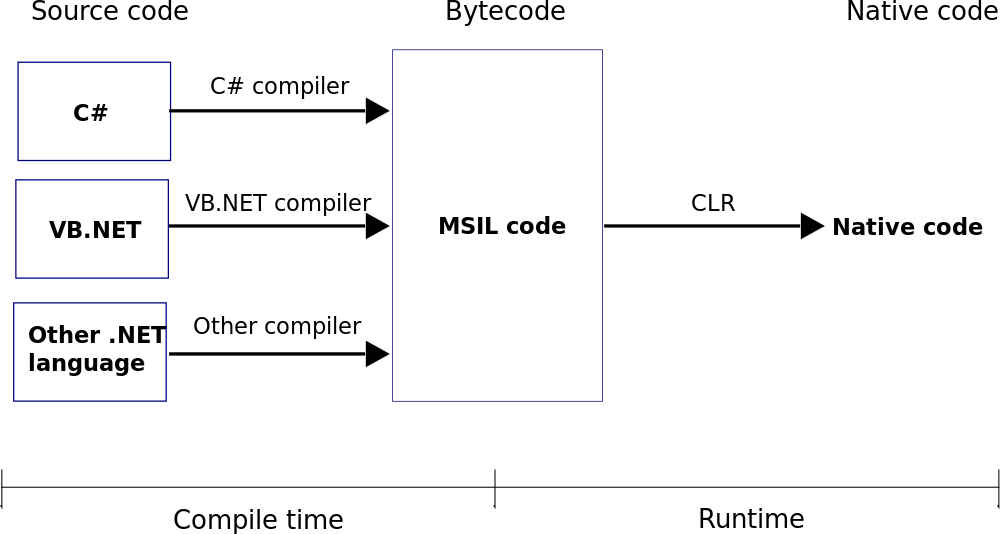
\includegraphics[width=15cm]{Csh_Imagenes/Compilacion.png}
\caption{Compilación en C\#}
\end{figure}
\section{Assemblies}
Los assemblies son los bloques de construcción de las aplicaciones del framework .NET. Un assembly es una colección de tipos y recursos que están construidos para trabajar en conjunto y formar la unidad lógica de la funcionalidad del programa.\\Todos los tipos en .NET Framework deben existir en assemblies; el tiempo de ejecución de idioma común no admite tipos fuera de ensamblados. Cada vez que crea una aplicación de Microsoft Windows, un servicio de Windows, una biblioteca de clases u otra aplicación con Visual Basic .NET, está creando un solo assembly. Cada assembly se almacena como un archivo .exe o .dll.\\Aunque es técnicamente posible crear assemblies que abarquen múltiples archivos, no es probable que use esta tecnología en la mayoría de las situaciones.\\.NET Framework usa assemblies como la unidad fundamental para varios propósitos:\\•Seguridad\\•Tipo de identidad\\•Versiones\\•Desarrollo

\chapter{Introducción a Visual Studio 2017 y C\# }
\section{Características de C\#}
C\# es un lenguaje de programación orientado a objetos, al ser posterior a C++ y Java. los lenguajes de programación orientados a objetos más conocidos hasta entonces, C\# combina y mejora gran parte de las características más interesantes de ambos lenguajes. Por tanto, un programador que conozca C\# a fondo no tendrá problemas para programar tanto en C++ como en Java, sus anteccesores.\\El nombre fue inspirado por la notación musical '\#' (llamada sostenido, en inglés Sharp) que indica que la nota es de un tono más alto. Se puede utilizar C\# para crear aplicaciones cliente de Windows, servicios Web XML, componentes distribuidos, aplicaciones cliente-servidor, aplicaciones de base de datos, y mucho, mucho más.\\Para poder crear programas en C\# y ejecutarlos posteriormente, es necesario tener instalado en el PC los siguientes paquetes:\\\\\textbf{.NET Framework SDK:} Es el kit de desarrollo e incluye un compilador de línea de C\# y bibliotecas que contienen una amplia colección de clases previamente definidas que podemos utilizar en nuestras aplicaciones; es decir, contiene todo lo necesario para poder crear y compilar nuestros programas.\\\textbf{.NET Framework Redistributable Package: } Permite la ejecución de programas creados en C\#. Esto es necesario porque la compilación de C\# no genera, como habitualmente para otros lenguajes, código máquina, sino un código escrito en un lenguaje propio de Microsoft: MSIL (Microsoft Intermediate Language). El CLR (Common Language Runtime) es el núcleo de la plataforma .NET y se encarga de gestionar la ejecución de los programas escritos en MSIL, ambos se pueden descargar gratuitamente desde la página web de la Red de Desarrolladores para Microsoft (Microsoft Developers Network) :\\ \textbf{https://www.microsoft.com/es-mx/download}\\\\También pueden crearse programas mediante la herramienta Visual Studio(Incluye en su instalación dichos paquetes), que ofrece un interfaz gráfico muy amigable y cómodo de utilizar, esta herramienta cuenta con una versión de paga y una gratuita (Community) y se puede descargar directamente desde la página oficial.\\\textbf{https://visualstudio.microsoft.com/es/}\\\\En la figura 2.2 se muestra un menú de paquetes complementarios que podemos descargar, si sólo queremos desarrollar en C\# basta con seleccionar los primeros dos paquetes.
\begin{figure}[hbtp]
\centering

\includegraphics[width=16cm]{Csh_Imagenes/Descarga1.png}
\caption{Página oficial para descargar Visual Studio}
\end{figure}
\begin{figure}[hbtp]
\centering
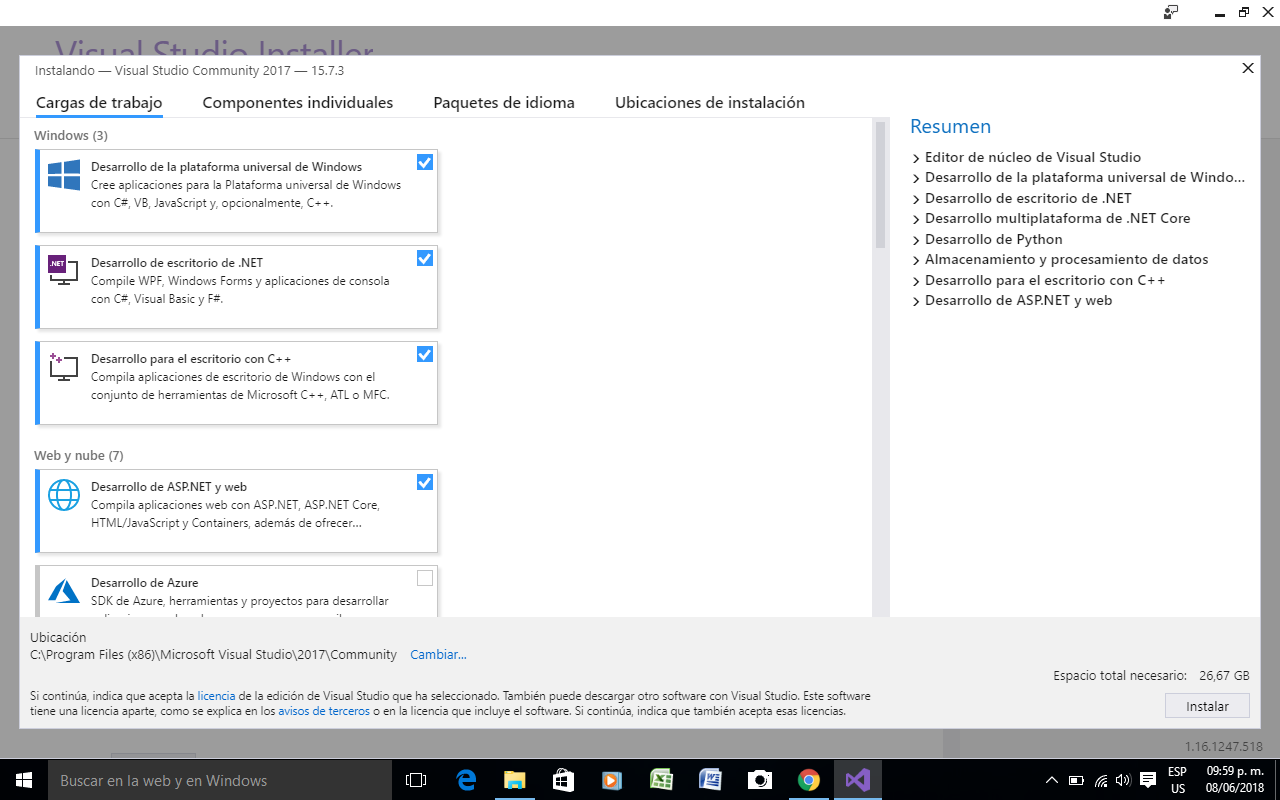
\includegraphics[width=16cm]{Csh_Imagenes/Instalacion.png}
\caption{}
\end{figure}
\section{Estructura de un programa}
Al abrir Visual Studio en la parte superior podemos observar un menú, para empezar un nuevo proyecto hacemos clic en la pestaña de Archivo, posteriormente seleccionamos la opción de nuevo y después proyecto, también podemos presionar la combinación de teclas Ctrl+Mayus+N. Se nos abrirá una ventana en la cual seleccionaremos la opción << Aplicacion de Consola >> y procedemos a darle un nombre a nuestro proyecto y damos click en aceptar. Ver las figuras 2.3 y 2.4.\\
\begin{figure}[hbtp]
\centering
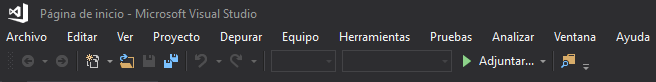
\includegraphics[width=16cm]{Csh_Imagenes/Menu_sup.PNG}
\caption{Menú superior en Visual Studio}
\end{figure}
\begin{figure}[hbtp]
\centering
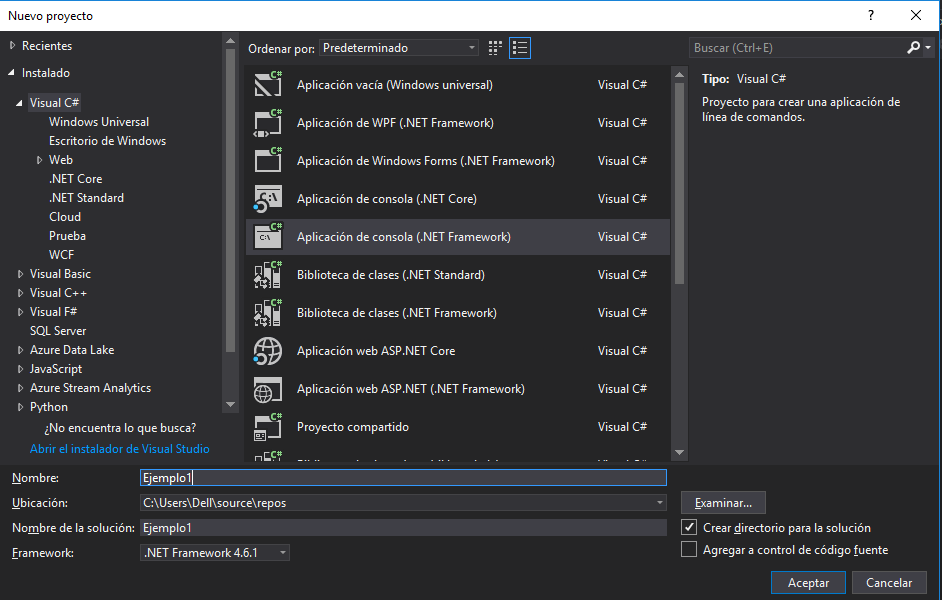
\includegraphics[width=16cm]{Csh_Imagenes/ConsoleApp.PNG}
\caption{}
\end{figure}
Para crear un proyecto sin Visual Studio necesitamos un editor de texto plano y los paquetes antes mencionados. Creamos una carpeta en el escrito llamada csharp, abrimos el block de notas y en este escribimos el código del ejemplo 1 con la extension \textit{.cs} y los guardamos dentro de la carpeta. Para poder compilar y ejecutar este programa necesitamos tener el comando \textit{csc} (el compilador de C\# incluido en la plataforma .NET) accesible. Para ello hay que modificar la variable de entorno Path, que contiene las carpetas en las que el sistema busca los programas a los que se invoca desde la línea de comandos. El proceso es el siguiente:\\\\\textbf{1.-} Buscar el lugar donde está instalada nuestra versión de .NET El Lugar por defecto es en una carpeta de la forma vXXXXX (donde XXXXX representa el número de versión de .NET que hemos instalado) que puede encontrarse en:\\\textbf{C:\textbackslash Windows\textbackslash Microsoft.NET\textbackslash Framework\textbackslash vX.X.XXXXX}\\\\\textbf{2.-} Abrir la cmd, esto se puede hacer abriendo el explorador y poner cmd o presionar la combinacion de las teclas Windows + R y escribir cmd. En la ventana de comandos escribir:\\\textbf{path=\%path\%;C:\textbackslash Windows\textbackslash Microsoft.NET\textbackslash Framework\textbackslash vX.X.XXXXX}.\\El comando \textit{csc} ya debe estar accesible desde la línea de comandos.\\\\C\# es un lenguaje orientado a objetos. En cualquier programa en C\# debe existir al menos una clase que contenga un método llamado \textbf{Main}. Este método constituye lo que se denomina punto de entrada, y define por dónde ha de comenzar a ejecutarse la aplicación: la primera instrucción ejecutada será la primera instrucción del método \textbf{Main}.\\El siguiente ejemplo muestra el programa más simple que puede crearse en C\#.\\\\

\textbf{Ejemplo 2.1}
\begin{lstlisting}
using System;
//Usamos el espacio de nombres System
class Ejemplo1 {
	static void Main() {
	
	}
}
\end{lstlisting}
Para crear una clase hay que escribir la palabra reservada \textbf{class} seguida del nombre que queremos darle. A continuación entre llaves, aparecerán los métodos y atributos de dicha clase. En este ejemplo hemos creado la clase \textit{Ejemplo 2.1}, que no incluye ningún atributo y contiene un solo método, de nombre \textbf{Main}. Como hemos dicho, todo programa en C\# debe contener al menos una clase con un método llamado \textbf{Main}.\\\\Es importante aclarar que C\# se distinguen las mayúsculas de las minúsculas, algo que no curre en todos los lenguajes de programación. Así, el punto de entrada ha de llamarse \textit{Main} y no \textit{main} o \textit{MAIN} o ninguna otra variante.\\\\Como para cualquier otro método existen varias alternativas válidas oara crear la declaración del método \textbf{Main}. Algunas son: \\\\\textit{public static int Main()\\public static void Main(string[] args)\\static int Main(string[] args)}\\\\La palabra \textbf{public} indica que el método es público, es decir, puede ser utilizado por otra clase (si no se pone nada, se considerará privado por defecto). La palabra \textbf{static} indica que que el método está asociado a la clase a la que pertenece y no a los objetos que se creen de dicha clase. En tercer lugar, aparece el tipo de la información que devuelve el método: \textbf{int} indica que devuelve un dato de tipo entero; \textbf{void}  indica que no se devuelve ningún valor. A continuación del nombre del método, que para el punto de entrada siempre es \textbf{Main}, aparecen entre paréntesis los argumentos o datos de entrada de este método, es decir, la información de la partida que requiere. Esta sección puede estar vacía.\\\\Por el momento dado los escasos conocimientos que aún tenemos, será suficiente con que el punto de entrada sea estático, no tenga argumentos y no devuelva ningún valor, tal y como se declaró en el ejemplo.
\section{Compilación y ejecución}
La compilación y ejecución usando Visual Studio resulta ser muy sencilla sin embrago se explicará el proceso con dicha herramienta y sin ella.\\Para compilar nos vamos al menú que se encuentra en la parte superior de la ventana de C\# y damos click en la pestaña donde dice Compilar, posteriormente se nos abrirá un menú en el cual seleccionaremos la opción de compilar solución. Al hacer dicho paso en la parte inferior aparecerá otra ventana conocida como la ventana de salida o de output donde se nos informará de todos los errores en nuestro programa antes de ejecutarlo. Una vez compilado nuestro programa nos vamos a la ventana superior y damos click en la pestaña donde dice depurar, al abrirse el menú seleccionamos la opción de iniciar sin depurar y se nos abrirá la ventana de comandos con nuestro programa en ejecución.\\Para compilar un programa sin Visual Studio nos vamos a la carpeta csharp creada en la sección pasada desde la cmd, para hacer esto abrimos la ventana de comandos y escribimos \textbf{cd c:\textbackslash csharp} y pulsamos intro, despues escribimos \textbf{csc Ejemplo1.cs} si sólo arroja un mensaje en el que nos indique la versión del compilador que se está utilizando, así como la version del Framework que está instalada significa que el código ha sido compilado con éxito, para ejecutar nuestro programa escribimos el nombre de éste sin la extensión .cs.


\chapter{Tipos predefinidos y control de flujo}
En este capitulo se mostrará cómo se utilizan datos de diferentes tipos básicos dentro de un programa y qué tipo de operaciones pueden realizarse con ellos.\\Normalmente, los programas sencillos necesitan de datos muy sencillos, pero los que conocemos hasta ahora son insuficientes. Por ejemplo, no podríamos plantearnos un programa que multiplique dos números enteros.\\\\Para manejar datos de tipos básicos cono enteros o reales, necesitamos dos cosas: poder almacenar esos datos en algún sitio, para lo que se utilizan variables, y poder manipular esos datos, para lo que necesitamos los operadores. Veremos a continuación qué tipos de datos tenemos disponibles en C\# y cuál es el conjunto de operadores que nos va a permitir transformar y operar con dichos datos.
\section{Tipos predefinidos de C\#}
El concepto de dato está relacionado con las operaciones que se pueden realizar sobre él. Un tipo de dato queda definido como un conjunto de valores que tienen asociadas una serie de operaciones para crearlos y manipularlos.\\\\En el ordenador cada tipo de datos se representa de una forma diferente. Una tabla parcial de los tipos que pueden manejarse en C\# se muestra en la figura 3.1
\begin{figure}[hbtp]
\centering
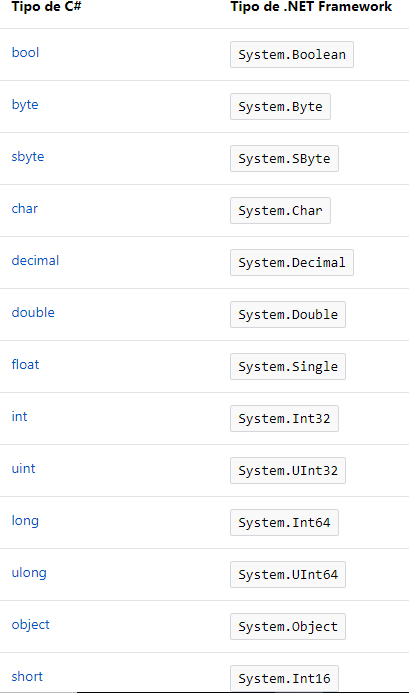
\includegraphics[width=8cm]{Csh_Imagenes/Tabla_Tipos.PNG}
\caption{Resumen del sistema de Tipos de C\#}
\end{figure}
\begin{figure}[hbtp]
\centering
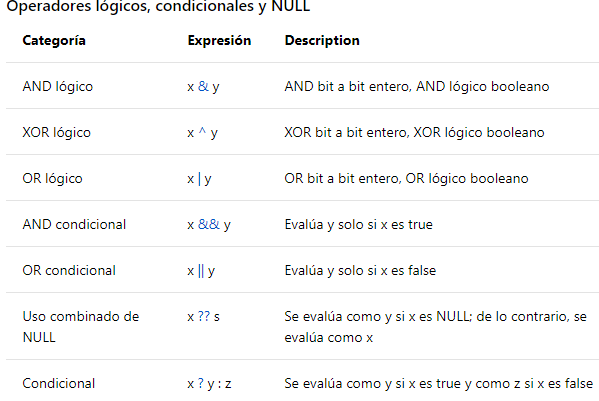
\includegraphics[width=16cm]{Csh_Imagenes/op_condicionales.PNG}
\caption{Operadores lógicos, condicionales y NULL}
\end{figure}
\begin{figure}[hbtp]
\centering
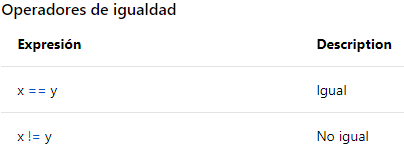
\includegraphics[width=16cm]{Csh_Imagenes/op_igualdad.PNG}
\caption{Operadores de igualdad}
\end{figure}
\begin{figure}[hbtp]
\centering
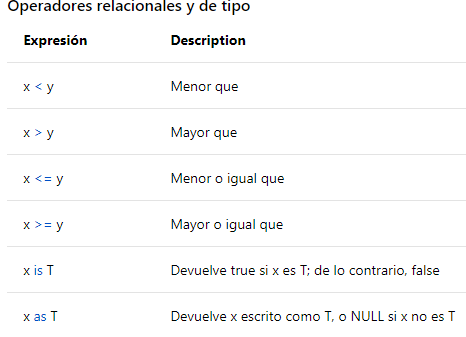
\includegraphics[width=16cm]{Csh_Imagenes/op_relacionales.PNG}
\caption{Operadores relacionales y de tipo}
\end{figure}

El nombre del tipo y la clase donde se define son, en realidad, la misma cosa. Es decir, el nombre del tipo es simplemente un alias y podemos utilizar indistintamente una u otro.\\\\Para aplicaciones grandes que manejan un gran volumen de datos es necesario optimizar el espacio que ocupan esos datos, ajustando lo máximo posible el tipo de las variables a los posibles valores que éstas vayan a almacenar.

\section{Tipos de referencia}
Hay dos clases de tipos en C\#: tipos de referencia y tipos de valor. Las variables de tipos de referencia almacenan referencias en sus datos (objetos), mientras que las variables de tipos de valor contienen directamente los datos. Con los tipos de referencia, dos variables pueden hacer referencia al mismo objeto y, por lo tanto, las operaciones en una variable pueden afectar al objeto al que hace referencia la otra variable. Con los tipos de valor, cada variable tiene su propia copia de los datos, y no es posible que las operaciones en una variable afecten a la otra .\\Las palabras clave siguientes se usan para declarar tipos de referencia:\\\textbf{class}: Palabra reservada para crear clases\\\textbf{Interface}: Una interfaz contiene solo las firmas de métodos, propiedades, eventos o indicadores.\\\textbf{delegate}: La declaración de un tipo delegado es similar a una firma de método. Tiene un valor devuelto y un número cualquiera de parámetros de cualquier tipo.
\section{Sentencias condicionales}
\textbf{Sentencia if}\\La sentencia \textbf{if} permite elegir entre dos alternativas en la función del valor(verdadero o falso) de cierta condición. Si la condición es verdadera, entonces se ejecuta un fragmento de código, y si es falsa, entonces se ejecuta otro distinto (usando la palabra else e indicando otro bloque de código), o no se ejecuta nada (No indicando el bloque de código else).
\textbf{Sintaxis de la instrucción if}.\\La instrucción \textbf{if} debe utilizarse de acuerdo a la siguiente sintaxis:
\begin{lstlisting}
if(<Condicion>)
  <instruccion_if>
else
  <instruccion_else>
\end{lstlisting}
\textbf{Ejemplo 3.1}\\
\begin{lstlisting}
using System;
class Ejemplo_3.1 {
  static void Main() {
    string nombre;  //Esta variable de tipo string guarda el nombre del usuario
    Console.WriteLine("Escribe tu nombre");
    nombre=Console.ReadLine();
    if(nombre == "Armando")
      Console.WriteLine("Bienvenido Armando!");
    else
      Console.WriteLine("Usuario no valido");   

    Console.ReadKey();  //Esta linea es util al ejecturar nuestro programa en Visua Studio para evitar que se cierre la consola inesperadamente.
  }
}
\end{lstlisting}
A menudo nos interesa introducir más de una línea de código en nuestros bloques \textbf{if}, \textbf{else} para esto utilizamos llaves {} en cada bloque.\\
\begin{lstlisting}
if(<Condicion>) {
  <instruccion1_if>
  <instruccion2_if>
  <instruccion3_if>
  <instruccion4_if>
}
else {
  <instruccion1_else>
  <instruccion2_else>
  <instruccion3_else>
}
\end{lstlisting}
En el ejemplo 2 la sentencia \textit{nombre == ``Armando"} regresa un valor y ese valor es \textbf{true} o \textbf{false}\\\\\textbf{La instrucción switch}\\
En ocaciones hay que tomar un gran número e decisiones dependiendo del valor que tiene una determinada expresión. Esto obliga a utilizar una colección de instrucciones \textbf{if} anidadas, tales que todas ellas realizan una comprobación sobre la misma expresión.\\\textbf{Sintaxis de la instrucción switch}\\La instrucción \textbf{switch} debe utilizarse de acuerdo a la siguiente sintaxis:\\
\begin{lstlisting}
switch (<expresion>) {
  case <valor1>: 
    <bloque_de_instrucciones_1>
    break;
  case <valor2>: 
    <bloque_de_instrucciones_2>
    break;
  ......
  case <valorn>: 
    <bloque_de_instrucciones_n>
    break;
  default:
    <bloque_de_instrucciones>
    break;
}
\end{lstlisting}
El significado de esta instrucción es la siguiente: se evalúa \textit{expresión}. Si su valor es \textit{valor1} se ejecuta \textit{bloque de instrucciones 1}, si es \textit{valor2} se ejecuta \textit{bloque de instruciones 2}, y así para el resto de valores especificados. Si no es igual a ninguno de esos valores y se incluye la rama \textbf{default}, se ejecuta \textit{<bloque de instrucciones>}; si no se incluye se pasa directamente a ejecutar la instrucción siguiente al \textbf{switch}.\\Los valores indicados en cada rama del \textbf{switch} han de ser expresiones constantes que produzcan valores de algún tipo básico. No puede haber más de una rama con el mismo valor. Cada bloque de instrucciones de cada rama debe terminar con una instrucción \textbf{break} para indicarle que continúe la ejecución con la siguiente instrucción al \textbf{switch}.
\\\textbf{Ejemplo 3.2}.
\begin{lstlisting}
using System;
class Ejemplo_Switch 
{
    static void Main()
    {
        Console.WriteLine("Cafes: 1=Chico 2=Mediano 3=Grande"); 
        Console.Write("Introduzca el cafe deseado: "); 
        string s = Console.ReadLine(); 
        int n = int.Parse(s); //Esta linea hace un casteo de cadena a un valor entero
        int cost = 0;
        switch(n)
        {
        case 1:
            cost += 25;
            break;
        case 2:
            cost += 50;
            break;
        case 3:
            cost += 75;
            break;
        default:
            Console.WriteLine("Seleccion invalida, Seleccione solo 1, 2, o 3.");
            break;
        }
        if (cost != 0)
        {
            Console.WriteLine("Introduzca {0} pesos.", cost);
        }
        Console.WriteLine("Gracias por su compra.");
    }
}
\end{lstlisting}
%Á á, É é, Í í,Ó ó,Ú ú,Ü ü,Ñ ñ, ¿, ¡ ``
\section{Ciclos de repetición}
\textbf{La instrucción while}\\Permite ejecutar un bloque de instrucciones mientras se cumpla una cierta condición: si la condición es verdadera, entonces se ejecuta el fragmento de código incluido dentro del \textbf{while}, y si es falsa, se salta el bucle y no se ejecuta nada.\\\textbf{Sintaxis de la instrucción while}\\La instrucción while debe utilizarse de acuerdo a la siguiente sintaxis.
\begin{lstlisting}
	while(<condicion>)
		<instrucciones>
\end{lstlisting}
\textbf{Ejemplo 3.3}.
\begin{lstlisting}
using System;
class Ejemplo_While 
{
    static void Main() {
    	int n = 0;
		while (n < 5) {
    		Console.WriteLine(n);
	    	n++;
		}
    }
}
\end{lstlisting}
Este ejemplo imprime los números del 0 al 4, es decir, el código se repite hasta que n sea menor a 5.\\\textbf{El bucle for}\\Un bucle for ejecuta un conjunto de declaraciones un número específico de veces y tiene la sintaxis.\\
\begin{lstlisting}
for(init; condicion; incremento;) {
	<Instrucciones>
}
\end{lstlisting}
Un contador es declarado una vez en \textbf{init}. A continuación, la \textbf{condicion} evalúa el valor del contador y el cuerpo del bucle es ejecutado si la condición es verdadera.\\Después de la ejecución del bucle, la declaración de \textbf{incremento} actualiza el contador, también llamado la variable de control del bucle.\\La condición es evaluada una vez más, y el cuerpo del bucle se repite, sólo deteniéndose cuando la condición se vuelve \textbf{falsa}.\\\textbf{Ejemplo 3.4}
\begin{lstlisting}
using System;
class Ejemplo_for {
	static void Main() {
		for(int x = 10; x < 15; x++) {
			Console.WriteLine("El valor de x es: " + x);		
		}
	}
}
\end{lstlisting}El anterior ejemplo imprime los números del 10 al 14\\En la última sección del \textbf{for} puede ir en lugar de x++ x+=3 o x-=2 dependiendo del interés del programador.\\Las declaraciones \textbf{init} e \textbf{incremento} pueden ser omitidas, si no se requieren, pero recuerda que los puntos y comas son obligatorios.\\\textbf{Ejemplo 3.5}\begin{lstlisting}
using System;
class Ejemplo_for {
	static void Main() {
	int x = 10;
		for(; x < 15; ) {
			Console.WriteLine("El valor de x es: " + x);
			x-=3;		
		}
	}
}
\end{lstlisting}El ciclo \textbf{for(;;){}} es un bucle infinito.\\\\
\textbf{El Bucle do-while}
Un bucle do-while es similar a un bucle \textbf{while}, excepto que un bucle \textbf{do-while} está garantizado a ser ejecutado al menos una vez.\\\\\textbf{Ejemplo 3.6}
\begin{lstlisting}
using System;
class Ejemplo_do_while {
	static void Main() {
	int x = 0;
		do {
			Console.WriteLine("El valor de x es: " + x);
			x++;		
		}while(x < 5);
	}
}
\end{lstlisting}Es muy importante colocar el \textbf{punto y coma} al final de la condición del \textbf{while}. si la condición del bucle \textbf{do-while} evalúa a \textbf{falso} las declaraciones en el \textbf{do} aún serán ejecutadas una vez. El bucle \textbf{do-while} ejecuta las declaraciones al menos una vez, luego valida la condición. El bucle \textbf{while} ejecuta la declaración sólo después de validar la condición.\\\\
\textbf{Ejemplo 3.7}
\begin{lstlisting}
using System;
class Ejemplo_do_while {
	static void Main() {
	int x = 42;
		do {
			Console.WriteLine("El valor de x es: " + x);
			x++;		
		}while(x < 10);
	}
}
\end{lstlisting}El ejemplo anterior imprime ``El valor de x es: 42" a pesar de que la condición del while no se cumpla.\\\\\textbf{Uso de break}\\Hemos visto el uso de \textbf{break} en la declaración \textbf{switch}.\\Otro uso de \textbf{break} es en los bucles: cuando la declaración \textbf{break} es encontrada. Dentro de un bucle, el bucle es terminado inmediatamente y la ejecución del programa es trasladada a la siguiente declaración que sigue al cuerpo del bucle.\\\\\textbf{Ejemplo 3.8}
\begin{lstlisting}
using System;
class Ejemplo_while {
	static void Main() {
	int x = 0;
		while (x < 20) {
			if(x == 5)
				break;
			Console.WriteLine("El valor de x es: " + x);
			x++;		
		}
	}
}
\end{lstlisting}El ejemplo anterior imprime los números del 0 al 4, si quitamos el break los imprimiría hasta el 19.\\Si estás utilizando bucles anidados (Un bucle dentro de otro), la declaración \textbf{break} detendrá la ejecución del bucle más interno y comenzará a ejecutar la siguiente línea de código después del bloque.\\\\\textbf{La declaración continue}\\La declaración \textbf{continue} es similar a la declaración \textbf{break}, pero en lugar de finalizar el bucle completamente, salta la iteración actual del bucle y continúa con la siguiente iteración.\\\\\textbf{Ejemplo 3.9}
\begin{lstlisting}
using System;
class Ejemplo_while {
	static void Main() {
		for(int i = 0; i < 10; i++) {
			if(i == 5)
				continue;
			Console.Writeline(i);		
		}	
	}
}
\end{lstlisting}El anterior ejemplo imprime los números del cero al nueve excepto el 5  ya que la declaración \textbf{continue} salta las declaraciones siguientes de esa iteración del bucle.

\chapter{Clases y Objetos}
\section{Conceptos básicos de POO}
C\# es un lenguaje que sigue el paradigma orientado a objetos, un paradigma en la programación representa un enfoque particular o filosofía para diseñar soluciones. Los paradigmas difieren unos de otros, en los conceptos y la forma de abstraer los elementos involucrados en un problema, así como en los pasos que integran su solución del problema, en otras palabras, el cómputo. También es importante definir que es una clase y que es un objeto.\\\textbf{Clase: }	La clase define un tipo de dato para un objeto pero no es un objeto en sí.\\\textbf{Objeto: }Un objeto es una entidad concreta basada sobre una clase y es llamado una instancia de una clase.\\\\La programación orientada a objetos está fundamentada sobre los cuatro pilares de la POO que son: \\\textbf{Abstracción: } La abstracción consiste en aislar un elemento de su contexto o del resto de los elementos que lo acompañan. En programación, el término se refiere al énfasis en el "¿Qué hace?" más que en el "¿Cómo lo hace?" por ejemplo \\\textbf{Encapsulamiento: }El encapsulamiento se refiere a restringir el acceso a las funciones internas de una clase.\\Beneficios:\\ - Controlar la manera en que los datos son accedidos o modificados.\\ - El código es mas flexible y fácil de cambiar a partir de nuevos requerimientos.\\ -  Poder modificar una parte del código sin afectar otras partes del mismo.\\\textbf{Herencia}: La herencia permite a la clase derivada reutilizar el código base sin tener que reescribirlo. Y la clase derivada puede ser personalizada añadiendo mas miembros.De esta manera, la clase derivada extiende la funcionalidad de la clase base.\\\textbf{Polimorfismo: }Significa “Tener muchas formas”. El polimorfismo es una forma de invocar el mismo método para diferentes objetos y generar diferentes resultados basados en el tipo de objeto.\\\\Estos conceptos los iremos trabajando a mayor profundidad en capítulos posteriores, sin embargo es importante tener una idea de su significado.\\\\Un programa construido mediante un lenguaje orientado a objetos no es más que una colección de objetos que se relacionan entre sí. La forma en que un objeto se comporta y las propiedades que lo definen dependen de la clase a la que pertenece.Una clase puede contener atributos que permiten definir información relativa a la clase y métodos que permiten manipular dichos atributos y definir el comportamiento de los objetos de la clase.\\\\Por ejemplo, mi \textit{coche} es un objeto de la clase \textit{automóvil} y como tal, tiene la capacidad de moverse a una \textit{velocidad constante}, de \textit{acelerarse}, de \textit{detenerse}, etc. Son atributos de mi \textit{coche}, entre otros, su \textit{marca} y \textit{modelo}, el \textit{número de matrícula}, la \textit{velocidad a la que viaja} en un momento dado y la \textit{cantidad de combustible} que lleva en el depósito. Como por ejemplo de métodos tendríamos \textit{arrancar}, \textit{acelerar}, \textit{frenar} y \textit{repostar}. Los métodos definen el modo en que funciona el objeto y pueden modificar ciertos atributos: \textit{repostar}, modificar la \textit{cantidad de combustible} mientras que \textit{acelerar} modifica, además de la \textit{cantidad de combustible}, la \textit{velocidad}.\\\\Cuando se crea un programa con un lenguaje orientado a objetos lo que se definen son las clases de todos los objetos que van a intervenir en el programa. Cuando dicho programa se ejecute, se crearán los objetos a medida que se necesiten, pudiendo haber más de un objeto de cada clase. Por ejemplo, un programa que se encarga de gestionar una biblioteca deberá contener muchos objetos de la clase libro (un objeto por cada ejemplar que existe en la biblioteca) y muchos objetos de la clase lector (uno por cada persona que utiliza dicha biblioteca). Cuando construimos el programa, únicamente creamos una clase libro y una clase lector, Durante el funcionamiento del programa (es decir, en tiempo de ejecución), se irán creando objetos de esas clases a medida que se necesiten, según se den de alta nuevos libros o nuevos usuarios.
\section{Creación de clases}
Una clase es una construcción que permite crear tipos personalizados propios mediante la agrupación de variables de otros tipos, métodos y eventos. Una clase es como un plano. Define los datos y el comportamiento de un tipo. Las clases se declaran mediante la palabra clave \textbf{class}.En Visual Studio das click derecho en \textbf{Proyecto} y en el submenú seleccionamos la opción \textbf{nuevo} y después \textbf{class}, automáticamente se crea un nuevo archivo con la estructura básica de una clase.    
\begin{lstlisting}
	public class Coche {
		//Campos, propiedades, atributos metodos.
	}
\end{lstlisting}
\section{Constructores}
Un \textsc{constructor} de clase en un miembro especial de una clase que es ejecutado cada vez que un nuevo objeto de esa clase es creado.\\Un \textsc{Constructor} tiene exactamente el mismo nombre que su clase, es público y no tiene ningún tipo de retorno. \\\textbf{Ejemplo 4.1:}\\
\begin{lstlisting}
	class Persona {
		private int edad;
		public Person() {
			Console.WriteLine("Hola amigo");		
		}	
	}
\end{lstlisting}Ahora, al momento de creación de un objeto del tipo Persona, el constructor es automáticamente invocado. Para hacer una objeto del tipo persona tenemos que especificar el nombre de la clase seguido de un identificador, posteriormente tenemos que hacer uso del operador de igualación y usar la palabra new como en el siguiente ejemplo.\\\textbf{Ejemplo 4.2}
\begin{lstlisting}
Using System;
	static void Main(string [] args) {
	Persona p = new Persona();	
	}
\end{lstlisting}La salida del código anterior es ``Hola amigo", 
\section{Propiedades}
Una propiedad es un miembro que ofrece un mecanismo flexible para leer, escribir o calcular el valor de un campo privado. Las propiedades proporcionan la comodidad de utilizar miembros de datos públicos sin los riesgos que implica el acceso no protegido y sin control ni comprobación a los datos de un objeto. Las propiedades pueden ser utilizadas como di fueran miembros públicos de datos, pero realmente incluyen métodos especiales llamados \textbf{descriptores de acceso (accessors)}\\El descriptor de acceso de una propiedad contiene las declaraciones ejecutables que ayudan a obtener (leer o computar) o fijar (escribir) un campo correspondiente. Las declaraciones del descriptor de acceso pueden incluir un descriptor de acceso \textbf{get}, un descriptor de acceso \textbf{set}, o ambas \\\textbf{Ejempo 4.3}
\begin{lstlisting}
class Persona {
	private string nombre;
	public string Nombre {
		get {return name; }
		set { nombre = value }	
	}
}
\end{lstlisting} La clase Persona tiene una propiedad \textbf{Nombre} que tiene tanto el descriptor de acceso \textbf{set} como el descriptor de acceso \textbf{get}.\\El descriptor de acceso set es utilizado para asignar un valor a la variable nombre mientras que get es utilizado para retornar su valor. \textbf{value} es una palabra clave especial, la cual representa el valor que asignamos a una propiedad utilizando el descriptor de acceso \textbf{set}. Una vez que la propiedad está definida, podemos utilizarla para asignar y leer el miembro privado.\\\textbf{Ejemplo 4.4 }
\begin{lstlisting}
class Persona {
	private string nombre;
	public string Nombre {
		get {return nombre; }
		set { nombre = value }	
	}
}

static void Main() {
	Persona p = new Persona();
	p.Name = "Armando";
	Console.WriteLine(p.name);
}
\end{lstlisting} La propiedad es accedida por su nombre, tal cual cualquier otro miembro público de la clase.\\Cualquier descriptor de acceso de una propiedad puede ser omitido. Por ejemplo, el siguiente código crea una propiedad que es sólo lectura: \\\textbf{Ejemplo 4.5}
\begin{lstlisting}
class Persona {
	private string nombre;
	public string Nombre {
		get {return nombre; }
	}
}
\end{lstlisting} Una propiedad puede también ser \textbf{privada}, por lo que sólo podrá ser invocada desde dentro de la clase. \\\\La utilidad de las propiedades es que tenemos la opción de controlar la lógica de acceso a la variable. Por ejemplo, puedes validar si el valor de \textbf{edad} es mayor que 0, antes de asignarlo a la variable:\\\textbf{4.6}
\begin{lstlisting}
class Persona {
	private string edad;
	public string Edad {
		get {return edad; }
		set { 		
			if(value > 0)			
			edad = value 
		}	
	}
}
\end{lstlisting} Cuando no necesitamos ninguna lógica personalizada, C\# provee un mecanismo rápido y efectivo para declarar miembros privados a través de sus propiedades.\\Por ejemplo, para crear un miembro privado que sólo pueda ser accedido a través de los descriptores de acceso \textbf{get} y \textbf{set} de la propiedad nombre, utiliza la siguiente sintaxis.
\begin{lstlisting}
public string Nombre {get; set;}
\end{lstlisting} Como puedes ver, no es necesario declarar el campo privado ``nombre" por separado.\\\textbf{4.7}
\begin{lstlisting}
class Persona {
	public string Nombre { get; set;}	
	}
}

static void Main() {
	Persona p = new Persona();
	p.Name = "Armando";
	Console.WriteLine(p.name);
}
\end{lstlisting} La salida del código anterior es ``Armando"
\section{Atributos y métodos de instancia}
Los atributos son todas aquellas características que le asociamos a un objeto de una clase definida.\\Los métodos representan todas aquellas acciones que puede realizar o se pueden llevar a cabo sobre un objeto de una clase.\\Los métodos de instancia son aplicables a una instancia de la clase en particular.\\También mediante el método constructor podemos pedir al usuario que indique la edad de la persona y esta será asignada al momento de hacer la instancia.\\\textbf{Ejemplo 4.8}
\begin{lstlisting}
class Persona {
	private int edad;
	public Person(int edad) {
		this.edad = edad;			
		Console.WriteLine("Hola amigo, tienes la edad de " + edad);		
	}
}
	
static void Main(string [] args) {
Persona p = new Persona(18);	
}
/*Salida: Hola amigo, tienes la edad de 18*/
\end{lstlisting} En el ejemplo anterior la palabra \textbf{this} hace referencia a la misma clase, es decir el parámetro recibido, en este caso 18, lo va a asignar al atributo edad. 
\section{Miembros estáticos}
Un miembro estático es aquel que pertenece a la propia clase en vez de a un objeto específico. El modificador static se utiliza para declarar los miembros de las clases(variables, métodos, propiedades) como estáticos.\\\textbf{Ejemplo 4.9}
\begin{lstlisting}
class Empleado {
	public static int contador = 0;
	public Empledo() {
		contador++;	
	}
}
\end{lstlisting} En este caso hemos declarado una variable miembro pública \textbf{contador}, la cual es \textbf{estática}. El constructor de la clase incrementa la variable \textbf{count} en uno.\\Sin importar cuantos objetos \textbf{Empleado} sean instanciados, siempre habrá una sola variable \textbf{count} que pertenece a la clase \textbf{Empleado} porque fue declarada \textbf{estática}.
\section{Estructuras}
Una estructura es un tipo de valor que normalmente se usa para encapsular pequeños grupos de variables relacionadas. Las estructuras también pueden contener constructores, constantes, campos, métodos, propiedades, eventos y tipos anidados. \\\textbf{Ejemplo 4.10}
\begin{lstlisting}
public struct Libro {
	public double precio;
	public string titulo;
	public string autor;
}

static void Main() {
	Libro l;
	l.titulo = "El retrato de Dorian Gray"
	l.precio = 100.00;
	l.autor = "Oscar Wilde"
	
	Console.WriteLine(l.titulo);
	/*Salida: El retrato de Dorian Gray*/
}
\end{lstlisting} Las estructuras no pueden heredar como las clases. Las clases se usan para modelar un comportamiento complejo, las estructuras tienen la intención principal de ser un conjunto simple de variables. Una clase es un tipo de referencia, un struct es un tipo de valor. Los campos no se puede inicializar a menos que sean constantes o estáticos. Una estructura puede implementar interfaces.
\section{Tipos de referencia vs Tipos de valor}
Un tipo de valor almacena su contenido en la memoria asignada en la pila. Cuando una variable de tipo de valor queda fuera de ámbito, porque en el método en que se definió ha finalizado la ejecución, el valor se descarta de la pila.
Por esto, es difícil compartir tipos de valor entre clases.\\\\C\# tiene dos formas de almacenar datos: por \textbf{referencia} y \textbf{por valor}.\\Los tipos de datos incorporados, como \textit{int} y \textit{double}, se utilizan para declarar variables que son tipos de \textbf{valor}. Su valor se almacena en la memoria en una ubicación llamada la \textbf{stack}.
Por ejemplo, la instrucción de declaración y asignación int x = 10; puede ser pensada como:
\begin{figure}[hbtp]
\centering
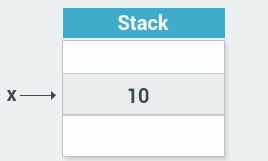
\includegraphics[width=6cm]{Csh_Imagenes/Stack.jpg}
\caption{Representación de la stack}
\end{figure}\\El valor de la variable x	 está ahora almacenada en la \textbf{stack}\\\\Los tipos de referencia se usan para almacenar objetos. Por ejemplo, cuando crea un objeto de una clase, se almacena como un tipo de referencia.
Los tipos de referencia se almacenan en una parte de la memoria llamada Heap.
Cuando crea una instancia de un objeto, los datos para ese objeto se almacenan en el montón, mientras que su dirección de memoria de montón se almacena en la pila.
Es por eso que se llama un tipo de referencia: contiene una referencia (la dirección de la memoria) al objeto real en el heap.\\Como puede ver en la figura 4.2, el objeto \textbf{p1} de tipo Persona en la stack almacena la dirección de memoria del heap donde está almacenado el objeto real.\\\textbf{Stack} se utiliza para la asignación de memoria estática, que incluye todos sus tipos de valores, como x.\\\textbf{Heap} se utiliza para la asignación de memoria dinámica, que incluye objetos personalizados, que pueden necesitar memoria adicional durante el tiempo de ejecución de su programa.\begin{figure}[hbtp]
\centering
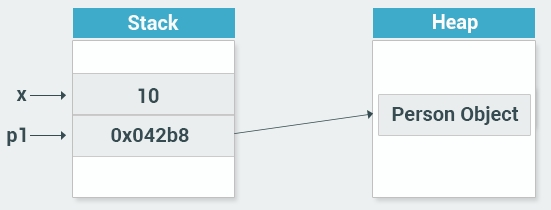
\includegraphics[width=10cm]{Csh_Imagenes/heap.jpg}
\caption{Representación de la Heap}
\end{figure}
\section{Clases estáticas}
Una clase estática es básicamente igual que una clase no estática, pero existe una diferencia: no se pueden crear objetos de una clase estática. El acceso a los miembros de una clase estática se realiza mediante el propio nombre de clase.\\Una clase estática es básicamente igual que una clase no estática, pero existe una diferencia: no se pueden crear objetos de una clase estática. El acceso a los miembros de una clase estática se realiza mediante el propio nombre de clase. Las clases estáticas:\\Sólo contiene miembros estáticos, no se pueden crear instancias de ella, es de tipo static, no puede contener constructores de instancia.\\\textbf{Ejemplo 4.11} \begin{lstlisting}
public static class Convertidor_Temperatura
{
    public static double Celsius_Fahrenheit(string temperaturaCelsius)
    {
        // Convierte el argumento a double para calcularlo.
        double celsius = Double.Parse(temperaturaCelsius);

        // Convierte Celsius a Fahrenheit.
        double fahrenheit = (celsius * 9 / 5) + 32;

        return fahrenheit;
    }

    public static double Fahrenheit_Celsius(string temperaturaFahrenheit)
    {
        // Convierte el argumento a double para calcularlo.
        double fahrenheit = Double.Parse(temperaturaFahrenheit);

        // Convierte Fahrenheit a Celsius.
        double celsius = (fahrenheit - 32) * 5 / 9;

        return celsius;
    }
}

class ConvertidorDeTemperatura
{
    static void Main()
    {
        Console.WriteLine("Seleccione una opcion para hacer la conversion");
        Console.WriteLine("1. Celsius a Fahrenheit.");
        Console.WriteLine("2. Fahrenheit a Celsius.");
        Console.Write(":");

        string opcion = Console.ReadLine();
        double F, C = 0;

        switch (opcion)
        {
            case "1":
                Console.Write("Ingrese la temperatura en Celsius: ");
                F =Convertidor_Temperatura.Celsius_Fahrenheit(Console.ReadLine());
                Console.WriteLine("Temperatura en Fahrenheit: {0:F2}", F);
                break;

            case "2":
                Console.Write("Ingrese la temperatura en Fahrenheit:  ");
                C =Convertidor_Temperatura.FahrenheitToCelsius(Console.ReadLine());
                Console.WriteLine("Temperatura en Celsius: {0:F2}", C);
                break;

            default:
                Console.WriteLine("Seleccione una opcion valida.");
                break;
        }
    }
}
/* Ejemplo:
	Seleccione una opcion para hacer la conversion
    1. Celsius a Fahrenheit.
    2. Fahrenheit a Celsius.
    :2
    Ingrese la temperatura en Fahrenheit: 20
    Temperatura en Celsius: -6.67
 */
\end{lstlisting}
Note que en el ejemplo anterior en ningún momento se está haciendo una instancia de la clase \textit{Convertidor\_Temperatura} debido a que es una clase estática.

\chapter{Control de Acceso}
\section{Namespaces}
El espacio de nombres permite agrupar varias clses que tienen cierta relación lógica entre ellas. Nosotros también podemos definir nuestros propios espacios de nombres, mediante la palabra reservada \textbf{namespace}, cada vez que escribimos al comienzo de un programa \textbf{using System}, estamos indicando a C\# que deseamos tener acceso a las clases definidas en el espacio de nombres \textbf{System}, entre las que se encuentran entre otras clases \textbf{Console} y \textbf{Math}.\\\textbf{Ejemplo 5.1}
\begin{lstlisting}
namespace Figuras {
	class Punto {
		// Atributos: coordenadas del punto en el plano
		private double x, y;
		//Constructor
		public Punto(double x, double y) {
			this.x = x;
			this.y = y;		
		}
		//Propiedades
		public double X {
			get {return x;}
			set { x = value;}
		}
		public double Y {
			get {return y;}
			set { x = y;}
		}
		//Suma a este punto las coordenadas del punto p
		public void suma(Punto p) {
			x += p.x;
			y += p.y;		
		} 
	} //Fin de la clase
} //Fin del espacio de nombres
\end{lstlisting}La clase \textsc{Punto} representa un punto situado sobre el plano. En la implementación hemos decidido que forme parte de un espacio de nombres \textsc{Figuras}. El método \textsc{suma} recibe un objeto de tipo \textsc{Punto} como argumento e incrementa las coordenadas del punto actual con las del argumento. El siguiente ejemplo muestra el uso de la clase anterior en un programa principal, para esto necesitamos utilizar el espacio de nombres \textsc{Figuras}.\\
\textbf{Ejemplo 5.2}
\begin{lstlisting}
using Figuras;
using System;
class Ejemplo5_2 {
	public static void Main() {
		Punto p = new Punto(1.0, 1.0);
		p.X(3.0);
		System.Console.WriteLine("x del punto: {0}, y del punto: {1}", p.X, p.Y);	
	}
}
\end{lstlisting}
\section{Encapsulamiento y modificadores de acceso}
Parte del significado de la palabra \textbf{encapsulación} es la idea de ``rodear" a una entidad, no solo para mantener lo que está dentro, sino también para protegerlo.\\En la programación, la \textbf{encapsulación} significa más que simplemente combinar miembros dentro de una clase; también significa restringir el acceso al funcionamiento interno de esa clase.\\La encapsulación se implementa mediante el uso de \textbf{modificadores de acceso}. Un modificador de acceso define el alcance y la visibilidad de un miembro de la clase.\\\\C\# admite los siguientes modificadores de acceso: \textbf{public}, \textbf{private},\textbf{ protected}, \textbf{internal}, \textbf{protected internal}.\\Como se vio en los ejemplos anteriores, el modificador de acceso \textbf{public} hace que el miembro sea accesible desde el exterior de la clase.\\El modificador de acceso \textbf{ private} hace que los miembros sean accesibles solo desde dentro de la clase y los oculta desde el exterior.\\\\\textbf{public}: Puede obtener acceso al tipo o miembro cualquier otro código del mismo ensamblado o de otro ensamblado que haga referencia a éste.\\\textbf{private}: Solamente puede obtener acceso al tipo o miembro código de la misma clase o struct.\\\textbf{protected}: Solamente puede obtener acceso al tipo o miembro el código de la misma clase o struct, o bien de una clase derivada de dicha clase.\\\textbf{internal}: Puede obtener acceso al tipo o miembro cualquier código del mismo ensamblado, pero no de un ensamblado distinto.\\\textbf{protected internal}: Puede obtener acceso al tipo o miembro cualquier código del ensamblado en el que se declara, o bien desde una clase derivada de otro ensamblado. El acceso desde otro ensamblado debe realizarse dentro de una declaración de clase derivada de la clase en la que se declara el elemento interno protegido y a través de una instancia del tipo de clase derivada.
\section{Métodos accesores vs propiedades}
Los métodos accesores o métodos \textbf{get} y \textbf{set} son métodos parecidos a las propiedades y nos sirven para tener un mejor control de nuestros atributos. \textbf{Ejemplo 5.3}
\begin{lstlisting}
namespace Figuras {
	class Punto {
		// Atributos: coordenadas del punto en el plano
		private double x, y;
		//Constructor
		public Punto(double x, double y) {
			this.x = x;
			this.y = y;		
		}
		//Metodos accesores
		public double getX() {
			return x;
		}
		public double getY() {
			return y;
		}
		public double setX(double x) {
			this.x = x;
		}
		public double setY(double y) {
			this.y = y;
		}
		//Suma a este punto las coordenadas del punto p
		public void suma(Punto p) {
			x += p.x;
			y += p.y;		
		} 
	} //Fin de la clase
} //Fin del espacio de nombres
\end{lstlisting}El uso es el mismo, sin embargo con las propiedades nos podemos ahorrar lineas de código. El siguiente ejemplo muestra el uso de la clase anterior en una clase principal.
\textbf{Ejemplo 5.4}
\begin{lstlisting}
using Figuras;
using System;
class Ejemplo5_4 {
	public static void Main() {
		Punto p = new Punto(1.0, 1.0);
		p.setX(3.0);
		System.Console.WriteLine("x del punto: {0}, y del punto: {1}", p.getX, p.getY);	
	}
}
\end{lstlisting}
\chapter{Arreglos}
\section{Sintaxis y uso de arreglos}
C\# proporciona numerosas clases integradas para almacenar y manipular datos.
Un ejemplo de dicha clase es la clase Array.\\Una \textbf{matriz},\textbf{array}, \textbf{vector} o \textbf{arreglo} es una estructura de datos que se usa para almacenar una colección de datos. Puedes pensarlo como una colección de variables del mismo tipo.\\Por ejemplo, considere una situación en la que necesite almacenar 100 números. En lugar de declarar 100 variables diferentes, puede declarar una matriz que almacena 100 elementos.\\Para declarar una matriz, especifique sus tipos de elementos entre corchetes:\\\textbf{Ejemplo 6.1}
\begin{lstlisting}
int[] miArreglo;
int[ ] miArreglo = new int[5]; /*Esta declaracion declara una matriz de enteros.Como las matrices son objetos, necesitamos instanciarlos con la nueva palabra new:*/
\end{lstlisting}Después de crear la matriz, puede asignar valores a elementos individuales usando el número de índice.\\\textbf{Ejemplo 6.2}
\begin{lstlisting}
int[] miArreglo = new int[5];
miArreglo[0] = 23; //Se agrega el numero 23 en el primer elemento del arreglo
\end{lstlisting}Note que los arreglos en C\# y en muchos otros lenguajes de programación el primer elemento es el índice cero, no uno como usualmente estamos acostumbrados a contar. Podemos inicializar un arreglo al momento de declararlo, o podemos omitir el tamaño del arreglo en la declaración si lo inicializamos, incluso podemos omitir el operador \textsc{new}. Podemos acceder a cada elemento especificando el indice de dicho elemento\\\textbf{Ejemplo 6.3}
\begin{lstlisting}
double[ ] precios = new double[4] {3.6, 9.8, 6.4, 5.9};
double[ ] precios = new double[ ] {3.6, 9.8, 6.4, 5.9};
double[ ] reales = {3.6, 9.8, 6.4, 5.9};

Console.WriteLine(reales[0]);	//Imprime 3.6
Console.WriteLine(reales[3]);	//Imprime 5.9
\end{lstlisting}A veces es necesario recorrer los elementos de una matriz, haciendo asignaciones de elementos basadas en ciertos cálculos. Esto se puede hacer fácilmente usando bucles.\\Por ejemplo, puede declarar una matriz de 10 enteros y asignarle a cada elemento un valor par con el siguiente ciclo:\\\textbf{Ejemplo 6.4}
\begin{lstlisting}
int[ ] a = new int[10];
for (int k = 0; k < 10; k++) {
  a[k] = k*2;
}
\end{lstlisting}También podemos usar un bucle para leer los valores de una matriz.\\Por ejemplo, podemos mostrar los contenidos de la matriz que acabamos de crear:\\\textbf{Ejemplo 6.5}
\begin{lstlisting}
for (int k = 0; k < 10; k++) {
  Console.WriteLine(a[k]);
}
\end{lstlisting}
\section{Arreglos multidimensionales}
Un Arreglo puede tener múltiples dimensiones, un Arreglo multidimensional es declarado de la siguiente forma.\\\textbf{Ejemplo 6.6}
\begin{lstlisting}
tipo[, , ... ,] Nombre_del_Arreglo = new tipo[size1, size2, ..., sizeN];
int[,]x = new int[3,4];
\end{lstlisting}En la figura 6.1 se ilustra un arreglo de 4x3.
\begin{figure}[hbtp]
\centering
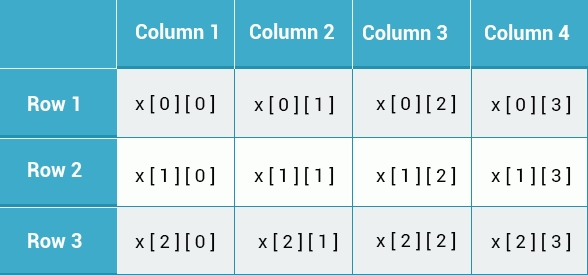
\includegraphics[width=10cm]{Csh_Imagenes/array.jpg}
\caption{Arreglo de 4x3}
\end{figure}También podemos inicializar los arreglos multidimensionales.\\\textbf{Ejemplo 6.7}
\begin{lstlisting}
int[ , ] Numeros = { {2, 3}, {5, 6}, {4, 6} }; 
\end{lstlisting}Esto creará una matriz con tres filas y dos columnas. Las llaves anidadas se usan para definir valores para cada fila.\\Para acceder a un elemento de la matriz, proporcione ambos índices. Por ejemplo, Numeros [2, 0] devolverá el valor 4, ya que accede a la primera columna de la tercera fila.\\Vamos a crear un programa que muestre los valores de la matriz en forma de una tabla.\\\textbf{Ejemplo 6.8}
\begin{lstlisting}
for (int k = 0; k < 3; k++) {
  for (int j = 0; j < 2; j++) {
    Console.Write(Numeros[k, j]+" ");
  }
  Console.WriteLine();
}
\end{lstlisting}Hemos utilizado dos ciclos for anidados, uno para iterar a través de las filas y otro a través de las columnas.\\\textit{Console.WriteLine ();} La instrucción mueve la salida a una nueva línea después de imprimir una fila.\\Las matrices pueden tener cualquier cantidad de dimensiones, pero tenga en cuenta que las matrices con más de tres dimensiones son más difíciles de administrar.\\\\Un \textit{jagged array} es una matriz cuyos elementos son matrices. Entonces, básicamente, es una matriz de matrices. La siguiente es una declaración de una matriz unidimensional que tiene tres elementos, cada uno de los cuales es una matriz de enteros de una sola dimensión:\\\textbf{Ejemplo 6.9}
\begin{lstlisting}
int[ ][ ] jaggedArr = new int[3][ ];
\end{lstlisting}Cada dimensión es una arreglo, por lo que también puedes inicializar el arreglo durante la declaración de la siguiente forma:\\\textbf{Ejemplo 6.10}
\begin{lstlisting}
int[ ][ ] jaggedArr = new int[ ][ ] {
  new int[ ] {1,8,2,7,9},
  new int[ ] {2,4,6},
  new int[ ] {33,42}
};
\end{lstlisting}Puedes acceder elementos individuales del arreglo como de muestra en el ejemplo siguiente:\\\textbf{Ejemplo 6.11}
\begin{lstlisting}
int x = jaggedArr[2][1]; //42
\\Accede al segundo elemento del tercer arreglo
\end{lstlisting}
Un \textbf{jagged array} es una matriz de arreglos, por lo que una int [] [] es una matriz de int [], cada una de las cuales puede tener diferentes longitudes y ocupar su propio bloque en la memoria.\\\textbf{Una matriz multidimensional} (int [,]) es un bloque único de memoria (esencialmente una matriz). Siempre tiene la misma cantidad de columnas para cada fila.
\section{Clase Array}
La clase Array en C\# proporciona varias propiedades y métodos para trabajar con matrices.\\Por ejemplo, las propiedades \textbf{Length} y\textbf{Rank} devuelven el número de elementos y el número de dimensiones de la matriz, respectivamente. Puede acceder a ellos usando la sintaxis de punto, al igual que cualquier miembro de la clase:\\\textbf{Ejemplo 6.12}
\begin{lstlisting}
int[ ] arr = {2, 4, 7};
Console.WriteLine(arr.Length); 
//Salida: 3
Console.WriteLine(arr.Rank); 
//Salida: 1
\end{lstlisting}La propiedad\textbf{ Length} puede ser útil en ciclos\textbf{ for} donde se necesita especificar el número de veces que se debe ejecutar el ciclo.\\\textbf{Ejemplo 6.12}
\begin{lstlisting}
int[ ] arr = {2, 4, 7};
for(int k=0; k<arr.Length; k++) {
  Console.WriteLine(arr[k]);
}
\end{lstlisting}Hay una serie de métodos disponibles para matrices.\\\textbf{Max} devuelve el valor más grande.\\\textbf{Min} devuelve el valor más pequeño.\\\textbf{Sum} devuelve la suma de todos los elementos.\\\textbf{Ejemplo 6.13}
\begin{lstlisting}
int[ ] arr = { 2, 4, 7, 1};
Console.WriteLine(arr.Max()); //Salida: 7
Console.WriteLine(arr.Min()); //Salida: 1
Console.WriteLine(arr.Sum()); //Salida: 14
\end{lstlisting}
\chapter{Objetos y métodos}
\section{Sobrecarga de métodos}
La sobrecarga de métodos se produce cuando varios métodos tienen el mismo nombre, pero diferentes parámetros.\\Por ejemplo, puede tener un método \textbf{Print} que muestre su parámetro en la ventana de la consola:\\\textbf{Ejemplo 7.1}
\begin{lstlisting}
void Print(int a) {
  Console.WriteLine("Valor: "+a);
}
\end{lstlisting}El operador + se usa para concatenar valores. En este caso, el valor de\textbf{ a} se une al texto ``Valor:".\\Este método solo acepta un argumento entero.\\Sobrecargarlo lo hará disponible para otros tipos, como el doble:\\\textbf{Ejemplo 7.2}
\begin{lstlisting}
void Print(double a) {
  Console.WriteLine("Valor: "+a);
}
\end{lstlisting}Ahora, el mismo nombre de método de impresión funcionará tanto para enteros como para dobles.\\Al sobrecargar los métodos, las definiciones de los métodos deben diferir entre sí por los tipos y/o el número de parámetros.\\Cuando hay métodos sobrecargados, el\textsc{ método} llamado se basa en los argumentos. Un \textsc{ argumento} \textbf{entero} llamará a la implementación del método que acepta un parámetro entero. Un argumento \textbf{double} llamará a la implementación que acepta un parámetro doble. Múltiples argumentos llamarán a la implementación que acepta la misma cantidad de argumentos.\\\textbf{Ejemplo 7.3}
\begin{lstlisting}
static void Print(int a) {
  Console.WriteLine("Valor: " + a);
}
static void Print(double a) {
  Console.WriteLine("Valor: " + a);
}
static void Print(string label, double a) {
  Console.WriteLine(label + a);
}

static void Main(string[] args) {
  Print(11);
  Print(4.13);
  Print("Promedio: ", 7.57);
}
\end{lstlisting}No puede sobrecargar las declaraciones de métodos que difieren solo por tipo de retorno.\\La siguiente declaración da como resultado un\textbf{ error}.\\\textbf{int} PrintName (int a) {}
\\\textbf{float} PrintName (int b) {}
\\\textbf{double} PrintName (int c) {}
\section{Comparación de objetos}
El problema de las referencias afecta también a la comparación de objetos, observe el siguiente código:\\\textbf{Ejemplo 7.4}
\begin{lstlisting}
Punto p1 = new Punto(0,0);
Punto p2 = new Punto(0,0);
//Comparamos
if(p1==p2)
	Console.WriteLine("Iguales");
else
	Console.WriteLine("Diferentes");
\end{lstlisting}Este fragmento de código escribe ``Diferentes" a pesar de que p1 y p2 representan ambos el mismo punto. La razón es porque las variables contienen referencias a los objetos: \textsc{p1} tiene una referencia a un objeto representando el punto (0,0) y \textsc{p2} tiene una referencia a un objeto representando el punto (0,0). El operador == no sirve para conocer si se trata de dos objetos iguales, sino si se trata de dos \textit{referencias} al mismo \textit{objeto}, y en este caso no lo son.\\\\Si queremos comparar el contenido de los objetos y no las referencias debemos escribir un método a propósito. Este método siempre se llama en C\# \textbf{Equals}, y es una buena idea incluirlo como miembro de todas las clases que definamos. La versión final de la clase \textsc{Punto} incluyendo el método \textbf{Equals} es la siguiente.\\\textbf{Ejemplo 7.5}
\begin{lstlisting}
namespace Figuras {
	class Punto {
		// Atributos: coordenadas del punto en el plano
		private double x, y;
		public Punto(double x, double y) {
			this.x = x;
			this.y = y;		
		}
		//Metodos accesores
		public double getX() {
			return x;
		}
		public double getY() {
			return y;
		}
		public double setX(double x) {
			this.x = x;
		}
		public double setY(double y) {
			this.y = y;
		}
		//Suma a este punto las coordenadas del punto p
		public void suma(Punto p) {
			x += p.x;
			y += p.y;		
		}
		public bool Equals(Punto p) {
			return x == p.getX && y == p.getY;		
		} 
	} //Fin de la clase
} //Fin del espacio de nombres
\end{lstlisting}Ahora podemos escribir el Ejemplo 7.4 y sí se escribirá el mensaje ``Iguales".
\section{Tipos anónimos}
Son una manera cómoda de encapsular un conjunto de propiedades de sólo lectura en un único objeto, Para crearlos se usa el operador \textbf{``new”} con un inicializador, no podemos saber de que tipo será nuestra variable, son datos por valor, es decir se crean en la pila y su referencia se pierde una vez terminado el método o estructura de control que lo haya creado. Son una forma conveniente de encapsular un conjunto de propiedades de solo lectura en un objeto, sin tener que crear una clase, son una instancia que no posee clase:
\textbf{Ejemplo 7.6}
\begin{lstlisting}
var persona = new {
	Nombre = "Marco",
	Apellido = "Aguilar"
}
\end{lstlisting}\textbf{var} significa que estamos dejando al compilador la tarea de asignar un tipo a nuestras variables.
\textbf{Ejemplo 7.7}
\begin{lstlisting}
// Define el tipo anonimo con new y un inicializador
var anonimo = new {
	Nombre = "LMD01",
	Precio = 1234.5,
	Serie = 2
};

// Mostrando los datos del objeto anonimo
	Console.WriteLine("Datos del objeto anonimo");
	Console.WriteLine(anonimo.Nombre);
	Console.WriteLine(anonimo.Precio);
	Console.WriteLine(anonimo.Serie);
	Console.ReadKey();
\end{lstlisting}
\section{Lista de parámetros variables}
C\# permite enviar a un método un número variable de parámetros mediante la palabra \textbf{``params”}. Sólo puede haber un parámetro\textbf{ params} por cada método.\\\textbf{Ejemplo 7.8}
\begin{lstlisting}
namespace ParametrosVariables {
	class Program {
		public static void UseParams(params int[] list) {
			for (int i = 0; i < list.Length; i++) {
				Console.Write(list[i] + " ");
			}
			Console.WriteLine();
		}

		public static void UseParams2(params object[] list) {
			for (int i = 0; i < list.Length; i++) {
				Console.Write(list[i] + " ");
			}
			Console.WriteLine();
		}

		static void Main(string[] args) {
			// Se puede especificar una lista separada por 
			//	comas del tipo especificado        
			UseParams(1, 2, 3, 4);
			UseParams2(1, 'a', "prueba");

			// params acepta cero o mas argumentos       
			UseParams2();

			// Se puede pasar un arreglo, mientras coincida con el
			//	tipo del parametro definido, en este caso int        
			int[] myIntArray = { 5, 6, 7, 8, 9 };
			UseParams(myIntArray);

			object[] myObjArray = { 2, 'b', "prueba", "hola" };
			UseParams2(myObjArray);

			// La siguiente linea genera un error de compilacion 
			//	porque un arreglo de object's no puede convertirse
			//	en un arreglo de enteros.
			//UseParams(myObjArray);
			// La siguiente llamada no causa error porque el arreglo
			//	de enteros se convierte en el primer y unico elemento
			//	de params            
			UseParams2(myIntArray, myIntArray);

			Console.ReadKey();
		}        
	}
}
\end{lstlisting}
\section{Modificadores de parámetros out y ref}
El modificador \textbf{out} indica que los argumentos se van a pasar por referencia. El modificador \textbf{ref}, es similar, sólo que éste requiere que se incialice la variable antes de pasarla.\\\\\textbf{Ejemplo 7.9}
\begin{lstlisting}
namespace OutRef
{
	class Program
	{
		public static void Main(string[] args)
		{
			String cadena = "Pedro", cadena2;

			Console.WriteLine(cadena);
			
			//Metodo Ref, recibe un argumento inicializado.
			MetodoRef(ref cadena);
			Console.WriteLine(cadena);
			
			//Metodo Out
			MetodoOut(out cadena2);
			Console.WriteLine(cadena2);
			
			Console.ReadKey(true);
		}
		
		public static void MetodoRef(ref String palabra){
			palabra = "Hola mundo";
		}
		
		public static void MetodoOut(out String frase){
			frase = "Te quiero";
		}
	}
}
\end{lstlisting}
\section{Llamada de parámetros con nombre}
La llamada de parámetros con nombre quita la necesidad de recordar o buscar el orden de los parámetros de los métodos. Es útil cuando se conocen los nombres de los parámetros:\\\\\textbf{Ejemplo 7.10}
\begin{lstlisting}
namespace ParametrosConNombre
{
	class Program
	{
		public static void Main(string[] args)
		{
			float weight, height, imc;
			
			//Pedimos estatura y peso al usuario
			Console.WriteLine("Ingresa tu peso en kilos: ");
			weight = float.Parse(Console.ReadLine());
			
			Console.WriteLine("Ingresa tu estatura en metros: ");
			height = float.Parse(Console.ReadLine());
			
			//Paso de parametros normal
			imc = IMC(weight, height);
			Console.WriteLine("El indice de masa corporal es: "+imc);
			
			//Paso de parametros con nombre
			imc = IMC(estatura:height, peso:weight);
			Console.WriteLine("El indice de masa corporal es: "+imc);
			
			//Lo que nunca se debe hacer
			//imc = IMC(estatura:height, weight);
			
			Console.ReadKey(true);
		}
		
		public static float IMC(float peso, float estatura){
			return peso/(estatura * estatura);
		}
		
	}
}
\end{lstlisting}
\chapter{Polimorfismo}
\section{Concepto de polimorfismo}
La palabra \textbf{polimorfismo} significa ``tener muchas formas". Normalmente, el polimorfismo ocurre cuando hay una jerarquía de clases y se relacionan a través de la\textbf{ herencia} de una clase base común.\\Polimorfismo significa que una llamada a un método miembro provocará que se ejecute una implementación diferente dependiendo del tipo de objeto que invoca el método.\\Simplemente, el polimorfismo significa que un único método puede tener varias implementaciones diferentes.\\\\Existen tres tipos de polimorfismo.\\\textbf{Polimorfismo por herencia}: cuando una clase hereda de otra y un objeto de la clase heredera puede ser tratado como un objeto de la clase padre.\\\textbf{Polimorfismos por abstracción}: cuando se hereda de una clase abstracta y el objeto creado también puede ser tratado como uno de esta clase abstracta.\\\textbf{Polimorfismo por interface}: es la posibilidad que tenemos de implementar una\textbf{ interface} y obtener un comportamiento en común de las clases que implementan la interfaz.\\El tema de Herencia se trata más a fondo en el siguiente capítulo.
\section{Interfaces y su implementación}
Una interfaz contiene las definiciones de un grupo de funciones relacionadas que una \textbf{clase} o\textbf{ struct} pueda implementar.\\ Mediante las interfaces, puede incluir, por ejemplo, comportamiento de varios orígenes en una clase. Esa función es importante en C\# porque el lenguaje no admite la herencia múltiple de clases.\\Una interfaz es una clase completamente abstracta, que contiene solo miembros abstractos. Se declara usando la palabra clave \textbf{interface}.\\Todos los miembros de la interfaz son abstractos por defecto, por lo que no es necesario utilizar la palabra clave abstract.\\Además, todos los miembros de una interfaz son siempre públicos, y no se les pueden aplicar modificadores de acceso.\\Es común usar la letra mayúscula I como la letra inicial para un nombre de interfaz.\\Las interfaces pueden contener propiedades, métodos, etc. pero no pueden contener campos (variables).\\Pero, ¿por qué usar interfaces en lugar de clases abstractas?\\Una clase puede heredar de solo una clase base, pero puede implementar múltiples interfaces.\\Por lo tanto, al usar interfaces, puede incluir el comportamiento de múltiples fuentes en una clase.\\Para implementar múltiples interfaces, use una lista de interfaces separadas por comas al crear la clase: clase A: IShape, IAnimal, etc.\\\\Características de las interfaces.\\Una interfaz es como una clase base abstracta. Cualquier clase o struct que implemente la interfaz debe implementar todos sus miembros.\\Una interfaz no puede ser instanciada directamente.\\Las interfaces pueden contener eventos, métodos, y propiedades.\\Una clase o struct puede implementar varias interfaces.\\\\La interfaz sólo contiene métodos vacíos (los agrumentos y los valores de retorno deben ser definidos). Implementa la interfaz y define los métodos.Implementa la interfaz y define los métodos de otra manera.\\\textbf{Ejemplo 8.1}
\begin{lstlisting}
public interface IPerro {
	string ladrar();
	string dormir();
}
public class Chihuahua : IPerro {
	public string ladrar() {
		return "Chihuahua ladrando"	
	}
	public string dormir() {
		return "Chihuahua durmiendo"	
	} 
}

public class Bulldog : IPerro {
	public string ladrar() {
		return "Bulldog ladrando"	
	}
	public string dormir() {
		return "Bulldog durmiendo"	
	} 
}
\end{lstlisting}Los dos puntos en las clases antes de \textit{IPerro} significan que esas clases van a hacer uso de la \textbf{interface} \textbf{IPerro} y están implementando sus métodos.\\\textbf{Ejemplo 8.2}
\begin{lstlisting}
namespace Polimorfismo {
    public interface IFigura {
        double CalcularArea();
    }
    
    public class Circulo : IFigura {
        public int Radio { get; set; }

        public double CalcularArea()
        {
            return Math.PI * Radio * Radio;
        }

        public void DatosCirculo()
        {
            Console.WriteLine("Radio: {0}", Radio);
        }
    }
    
    public class Rectangulo : IFigura {
        public int Base { get; set; }
        public int Altura { get; set; }

        public double CalcularArea()
        {
            return Base * Altura;
        }

        public void DatosRectangulo()
        {
            Console.WriteLine("Base: {0}, Altura: {1}", Base, Altura);
        }
    }
    
    public class Triangulo : IFigura {
        public int Base { get; set; }
        public int Altura { get; set; }

        public double CalcularArea()
        {
            return Base * Altura / 2;
        }

        public void DatosTriangulo()
        {
            Console.WriteLine("Base: {0}, Altura: {1}", Base, Altura);
        }
    }
    
    class Program {
        static void Main(string[] args) {
            // Upcasting
            IFigura f1 = new Circulo { Radio = 5 };            
            IFigura f2 = new Triangulo { Base = 10, Altura = 8 };
            IFigura f3 = new Rectangulo { Base = 4, Altura = 3 };
            IFigura f4 = new Circulo { Radio = 9 };

            IFigura[] figuras = new IFigura[] { f1, f2, f3, f4 };

            foreach (var figura in figuras) {
                Console.WriteLine(figura.CalcularArea());
            }

            // Dowcasting
            Circulo c = f1 as Circulo;
            Console.WriteLine("Datos del circulo");
            c.DatosCirculo();
        }
    }
}
\end{lstlisting}
\section{Relación de subtipos y supertipos}

\chapter{Herencia}
\section{Herencia (is-a relationship)}
\section{Métodos virtuales}
\section{Palabras reservadas virtual y override}
\section{Clases abstractas y clases selladas}
\section{Clase Object}

\part{C\# Intermedio}

\chapter{Excepciones}
\section{Clase Exception}
\section{Bloque try-catch-finally}
\section{Definición de una excepción}
\section{Relanzar Excepciones}

\chapter{Strings}
\section{String vs StringBuilder}
\section{Formato de una cadena}
	
\chapter{Manejo de archivos}
\section{Archivos y flujos}
\section{Manejo de sistema de archivos}
\section{Clases File, FileInfo, Directory, DirectoryInfo}
\section{Lectura y escritura de archivos}

\chapter{Genéricos}
\section{Necesidad de tipos genéricos}
\section{Métodos genéricos}
\section{Clases genéricas}

\chapter{Colecciones}
\section{Listas y Diccionarios}

\chapter{Concurrencia}
\section{Clases Thread y Parallel}
\section{Tasks}
\section{Sincronización}

\chapter{Lambdas, Delegados y Eventos}
\section{Expresiones Lambda}
\section{Introducción a delegados y eventos}
\section{Creación y uso de delegados}
\section{Multicast delegate}
\section{Uso de eventos}
\section{Clase EventArg}

\chapter{LINQ (Checar Entity Framework)}
\section{Introducción a LINQ}
\section{Query syntax}
\section{Métodos de extensión}
\section{Operaciones estándar de consulta}

\part{C\# Avanzado}
\chapter{ Interfaces gráficas de usuario con Windows Forms}
\section{Introducción a las GUIs}
\section{Manejo básico de eventos}
\section{Propiedades de los controles y Layouts}

\chapter{Controles de Windows Forms}
\section{Labels, TextBox y Buttons}
\section{GroupBox y Panel}
\section{CheckBox y RadioButton}
\section{PictureBox}
\section{ToolTips}
\section{MouseEvents y KeyboardEvents}
\section{ProgressBar}
\section{Menu}
\section{MonthCalendar}
\section{DataTimePicker}
\section{LinkLabel}
\section{ListBox, CheckedListBox y ComboBox}
\section{ListView}
\section{TabControl}
\section{Chart}

\chapter{Introducción a Programación Asíncrona}
\section{Métodos asíncronos}
\section{Palabras async y await}

\chapter{WPF (Windows Presentation Foundation)}
\section{¿Qué es WPF?}
\section{Diferencias entre WPF y Windows Forms}
\section{Mi primera aplicación con WPF}

\chapter{Bases de datos con LINQ}
\section{Introducción a las bases de datos relacionales}
\section{LINQ to Entities y ADO.NET}
\section{Operaciones CRUD}

\chapter{Control de versiones con Team Explorer y Git}
\section{Configuración de Git y Team explorer}
\section{Manejo de ramas}
\section{Commit}
\end{document}

%Á á, É é, Í í,Ó ó,Ú ú,Ü ü,Ñ ñ, ¿, ¡ ``